% --------------------------------------------------------------
% This is all preamble stuff that you don't have to worry about.
% Head down to where it says "Start here"
% --------------------------------------------------------------
 
\documentclass[12pt]{article}

\usepackage{courier}
\usepackage{color}
\usepackage{listings}
\usepackage[square,numbers]{natbib}
\usepackage{tabls}
\usepackage{graphicx}
\usepackage{subcaption}
\usepackage{pdfpages}
\usepackage{mathtools}

\definecolor{dkgreen}{rgb}{0,0.6,0}
\definecolor{gray}{rgb}{0.5,0.5,0.5}




\lstset{language=python,
   basicstyle=\ttfamily,
   keywordstyle=\color{blue},
   commentstyle=\color{dkgreen},
   stringstyle=\color{red},
   numbers=left,
   numberstyle=\tiny\color{gray},
   stepnumber=1,
   numbersep=10pt,
   backgroundcolor=\color{white},
   tabsize=4,
   showspaces=false,
   showstringspaces=false}
 
\usepackage[margin=1in]{geometry} 
\usepackage{amsmath,amsthm,amssymb}
\usepackage{verbatim}
\usepackage{algpseudocode,algorithm}
\usepackage{setspace}

\newcommand{\ihat}{\ensuremath{\hat{\textbf{\i}}}}
\newcommand{\jhat}{\ensuremath{\hat{\textbf{\j}}}}
\newcommand{\lline}{\noindent\makebox[\linewidth]{\rule{\textwidth}{0.4pt}}}
\newcommand{\N}{\mathbb{N}}
\newcommand{\Z}{\mathbb{Z}}
\newcommand{\deriv}[2]{\frac{\mathrm{d} #1}{\mathrm{d} #2}}
\newcommand{\pderiv}[2]{\frac{\partial #1}{\partial #2}}
\newcommand{\bx}{\mathbf{X}}
\newcommand{\ba}{\mathbf{A}}
\renewcommand{\d}{\mathrm{d}}
\newcommand{\upl}{u_{\text{plane}}}
\newcommand{\upt}{u_{\text{point}}}
\newcommand{\D}{\Delta}
\newcommand{\ra}{\rightarrow}
\renewcommand{\SS}{\State}
 
\newenvironment{theorem}[2][Theorem]{\begin{trivlist}
\item[\hskip \labelsep {\bfseries #1}\hskip \labelsep {\bfseries #2.}]}{\end{trivlist}}
\newenvironment{lemma}[2][Lemma]{\begin{trivlist}
\item[\hskip \labelsep {\bfseries #1}\hskip \labelsep {\bfseries #2.}]}{\end{trivlist}}
\newenvironment{exercise}[2][Exercise]{\begin{trivlist}
\item[\hskip \labelsep {\bfseries #1}\hskip \labelsep {\bfseries #2.}]}{\end{trivlist}}
\newenvironment{problem}[2][Problem]{\begin{trivlist}
\item[\hskip \labelsep {\bfseries #1}\hskip \labelsep {\bfseries #2:}]\hspace{0.3in}\newline\newline}{\end{trivlist}}
\newenvironment{question}[2][Question]{\begin{trivlist}
\item[\hskip \labelsep {\bfseries #1}\hskip \labelsep {\bfseries #2.}]}{\end{trivlist}}
\newenvironment{corollary}[2][Corollary]{\begin{trivlist}
\item[\hskip \labelsep {\bfseries #1}\hskip \labelsep {\bfseries #2.} ]}{\end{trivlist}}
\newenvironment{problem*}[1][Problem]{\begin{trivlist}
\item[\hskip \labelsep {\bfseries #1} {\hspace{-0.2em}\bfseries:}]}{\end{trivlist}}
\newenvironment{solution}[1][Solution]{\begin{trivlist}
\item[\hskip \labelsep {\bfseries #1} {\hspace{-0.2em}\bfseries:}]\hspace{0.3in}\newline}{\end{trivlist}}
 
\begin{document}
 
% --------------------------------------------------------------
%                         Start here
% --------------------------------------------------------------
 
\title{Homework 1}%replace X with the appropriate number
\author{Simon Bolding\\ %replace with your name
NUEN 629} %if necessary, replace with your course title
 
\maketitle

\clearpage

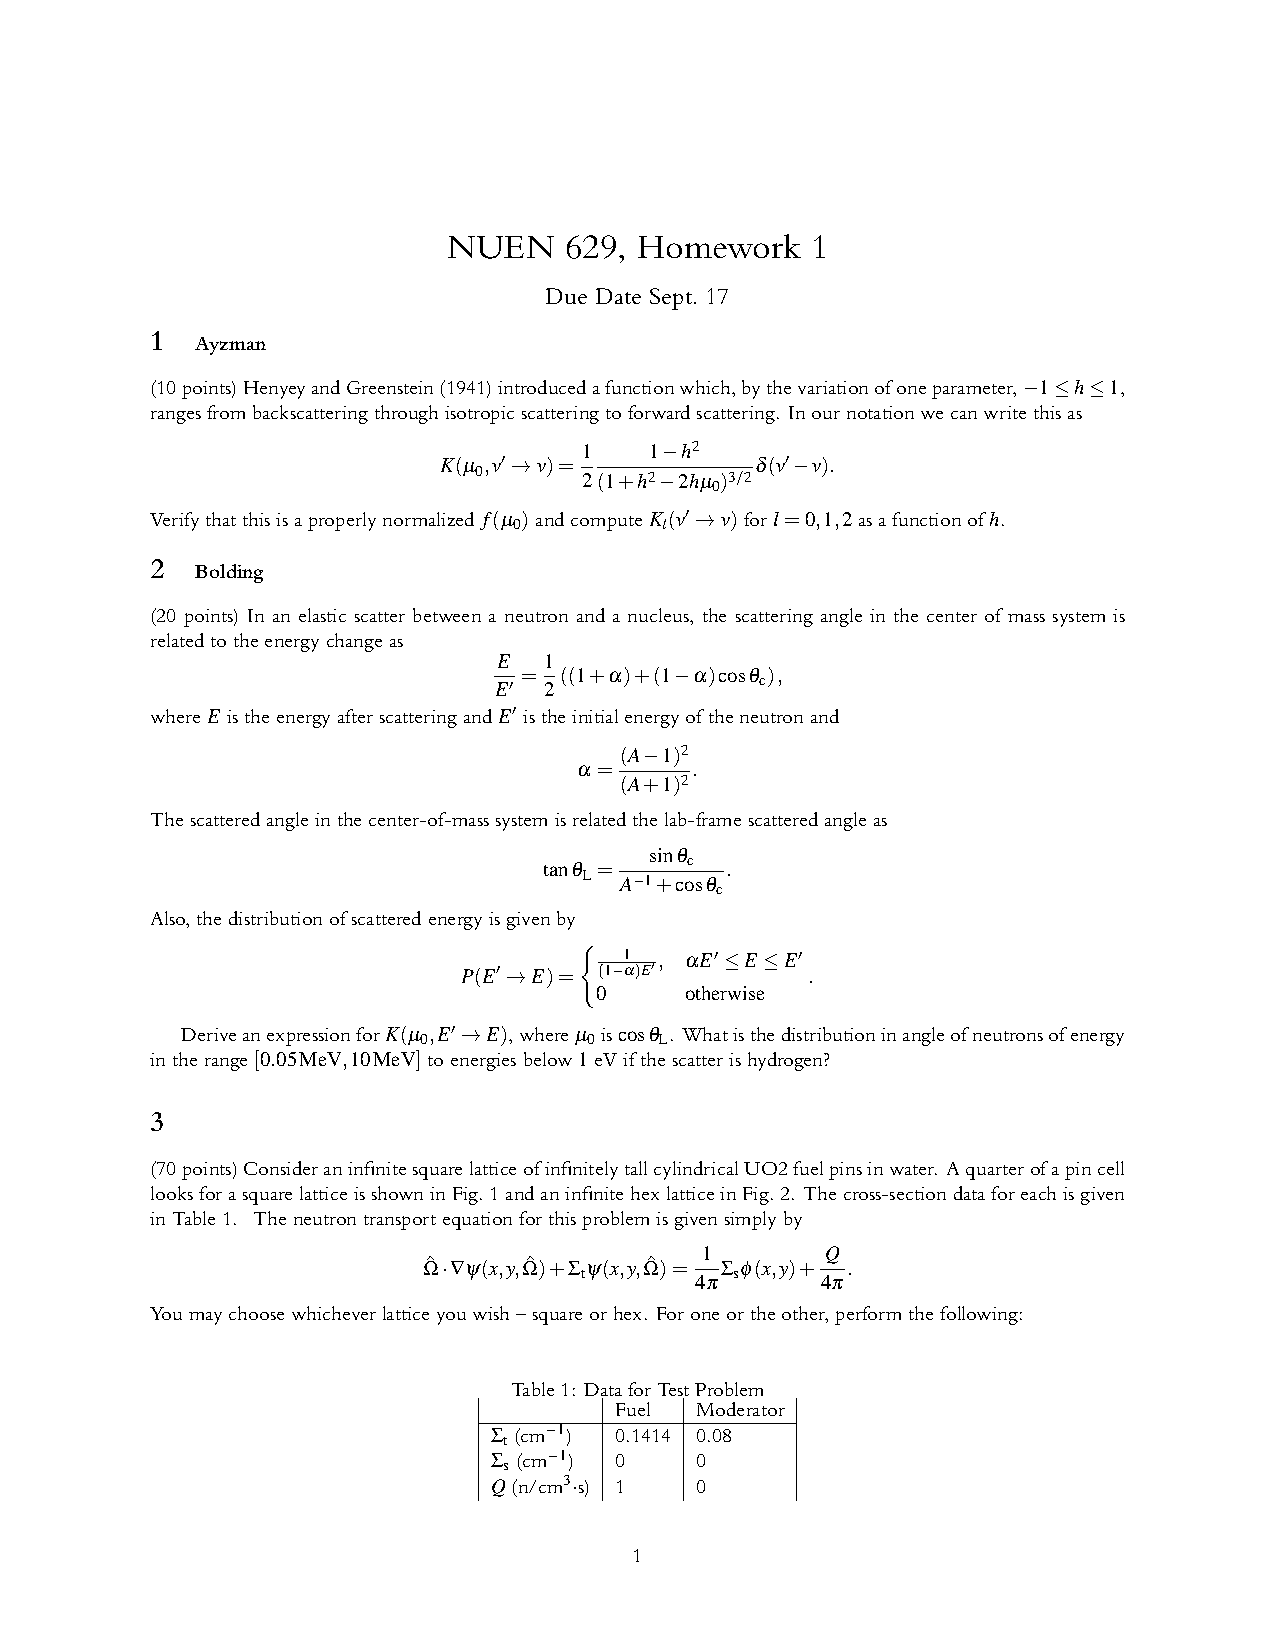
\includepdf[pages={1-3}]{Homework1.pdf}

%\includepdf[pages={1}]{p1p3.pdf}

\begin{problem}{1}
Henyey and Greenstein (1941) introduced a function which, by the variation of one
parameter, $−1 \leq h \leq 1$, ranges from backscattering through isotropic scattering to forward scattering. In
our notation we can write this as
\begin{equation}
    K( \mu_0 , v'\rightarrow v) = \frac{1}{2}
    \frac{1-h^2}{\left(1+h^2-2h\mu_0\right)^{3/2}}\delta(v'-v).
\end{equation}
Verify that this is a properly normalized $f ( \mu_0 )$ and compute $K_l (v'
\rightarrow → v)$ for $l = 0, 1, 2$ as a function of $h$.

\end{problem}

\begin{solution}
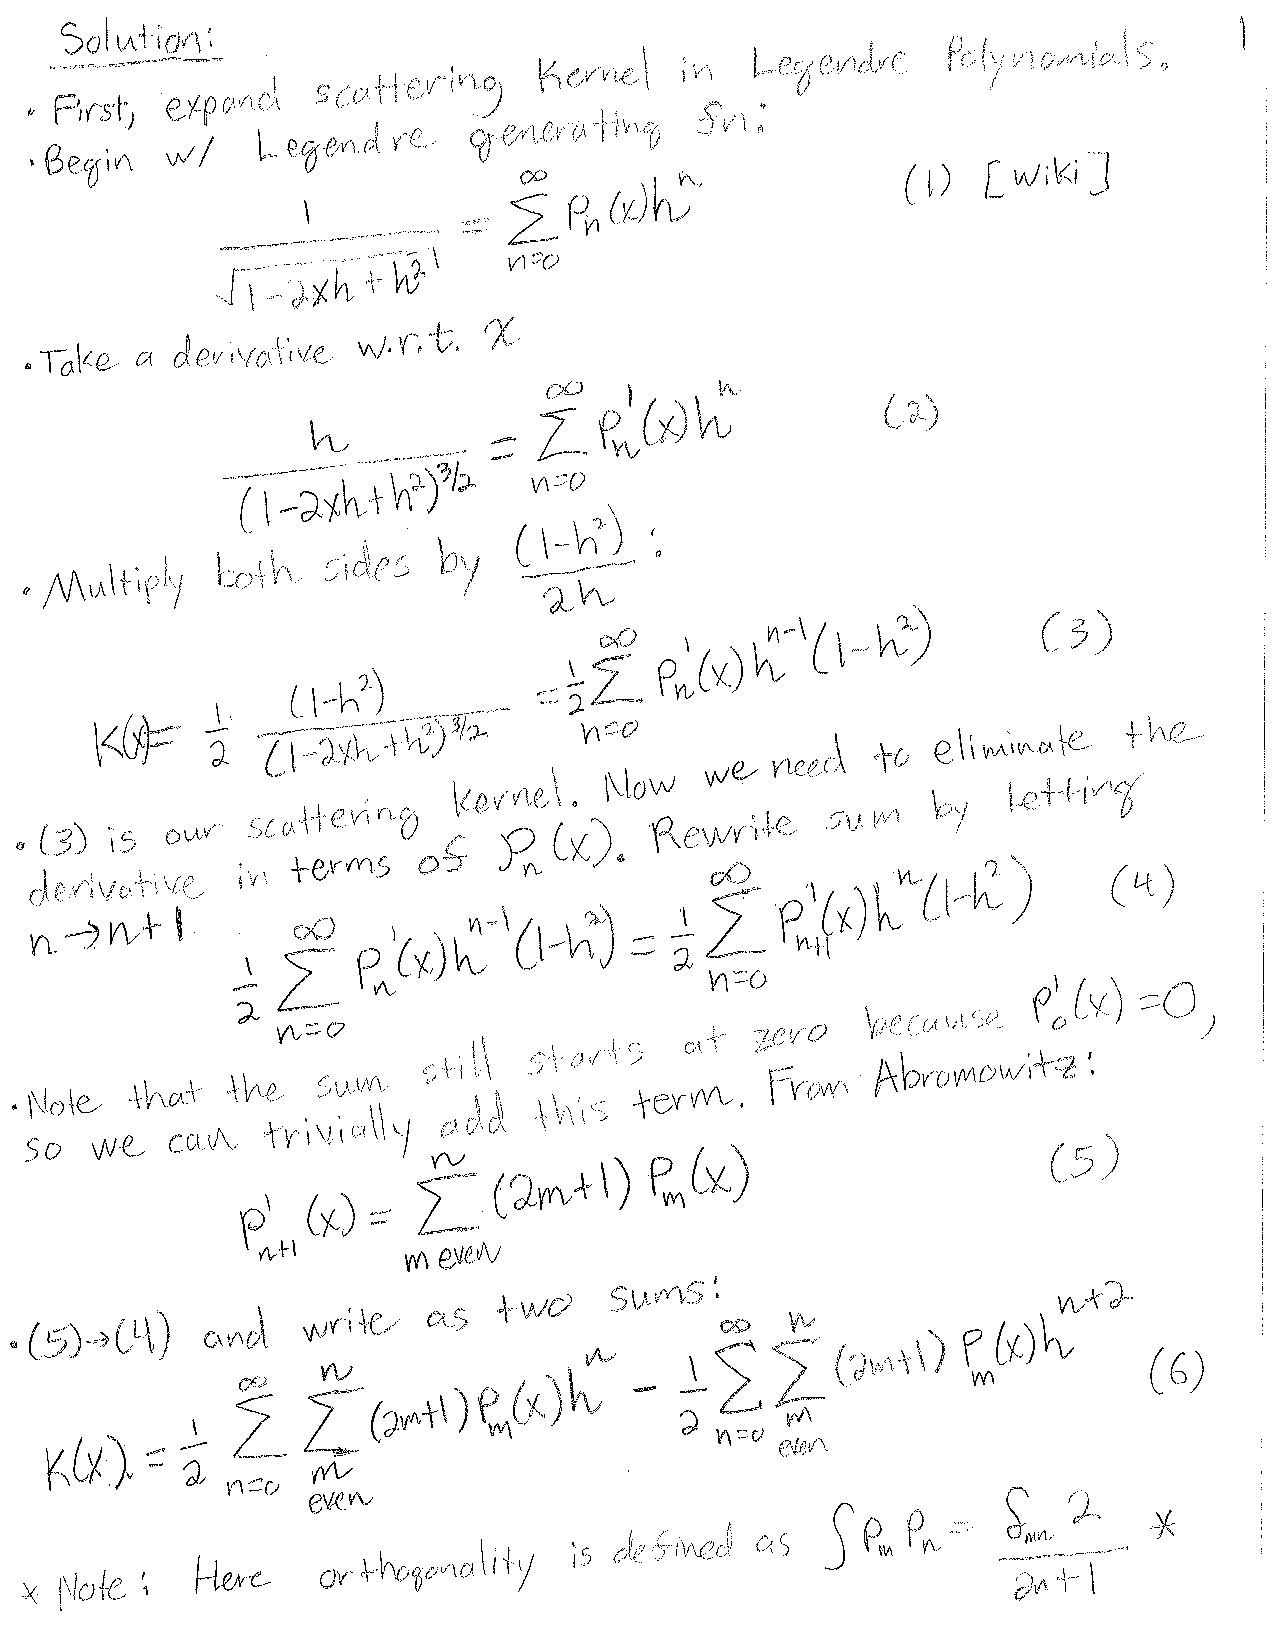
\includepdf[pages={1-2}]{p1.pdf}
\end{solution}
\clearpage

\begin{problem}{2}
In an elastic scatter between a neutron and a nucleus, the scattering angle in the center of mass system is
related to the energy change as
\begin{equation}\label{eq:E}
 \frac{E}{E'} = \frac{1}{2}\left((1+\alpha) + (1-\alpha)\cos \theta_c\right)
\end{equation}
where $E$ is the energy after scattering and $E'$′ is the initial energy of the neutron and
\begin{equation}
\alpha = \frac{(A-1)^2}{(A+1)^2}.
\end{equation}
The scattered angle in the center-of-mass system is related the lab-frame scattered angle as
\begin{equation}\label{eq:tan}
\tan \theta_L = \frac{A\sin \theta_c}{1 + A\cos \theta_c}
\end{equation}
Also, the distribution of scattered energy is given by
\begin{equation} \label{pdf}
P(E'\rightarrow E) = \left\{\begin{matrix}
\frac{1}{(1-\alpha)E'} & E'\alpha \leq E \leq E' \\ 
 0 & \text{otherwise}
\end{matrix}\right. .
\end{equation}
Derive an expression for $K( \mu_0, E'\rightarrow E)$, where $\mu_0$ is $\cos \theta_L$. What is the distribution in angle of neutrons of energy
in the range [0.05 MeV, 10 MeV] to energies below 1 eV if the scatter is with hydrogen?

\end{problem}

\begin{solution}

    \subsubsection*{Scattering Kernel Derivation}

Due to Eq.~\eqref{eq:E}, for a fixed $A$, a given value of $E$ and $E'$ fully define
$\mu_c$; the lab frame cosine of the scattering angle $\mu_0$ is also fully defined through
Eq.~\eqref{eq:tan}.  As a result, the shape of the doubly differential scattering cross section
 is fully defined by the probability density function (PDF) $P(E'\ra E)$. Thus, it is
possible to write the scattering cross section in the COM frame as~\cite{dunnshultis}
\begin{equation}
    \Sigma_s(\mu_0,E'\ra E) = \Sigma_s(E')P(E' \ra E) \delta(\mu_c - f_\mu(E,E'))
 \end{equation}
 where $f_\mu(E,E')$ is the value of $\mu_c$ that satisfies Eq.~\eqref{eq:E} for a given
 $E$, i.e.,
 \begin{equation}
     f_\mu(E,E') = \frac{2(\frac{E}{E'}) - (1+\alpha)}{(1-\alpha)}
 \end{equation}
Because we are interested in the scattering kernel as a function of the lab frame
cosine $\mu_0$, 
we define the scattering cross section in an equivalent form 
 \begin{equation}
     \Sigma_s(\mu_0,E'\ra E) = \Sigma_s(E')P(\mu_0)\delta(E - f_{E}(\mu_c(\mu_0),E'))
 \end{equation}
 where $P(\mu_0)$ is a PDF for $\mu_0$ given a certain value of $E'$, $f_E$ is
 defined as
 \begin{equation}
  f_E(\mu_C,E') = \frac{E'}{2}\left((1+\alpha) + (1-\alpha)\mu_c\right),
 \end{equation}
 and $\mu_c$ as a function of $\mu_0$ will be derived later in Eq.~\eqref{eq:muc}. The scattering kernel is defined as
 \begin{equation}
     K(\mu_0,E'\ra E) = \frac{\Sigma_s(E'\ra E,\mu_0)}{\displaystyle\int\limits_{0}^\infty\d
     E\!\int\limits_{-1}^1 \d \mu_0\,
 \Sigma_s(E'\ra E,\mu_0)}
 \end{equation}
 The denominator is evaluated as
 \begin{equation}
     \int\limits_{-1}^1 \!\d \mu_0 \int\limits_0^\infty \!\d E \;
     \Sigma_s(E')P(\mu_0)\delta(E-f_{E}(\mu_c(\mu_0),E)) =
     \Sigma_s(E')\int\limits_{-1}^1 \d\mu_0 P(\mu_0) = \Sigma_s(E')
 \end{equation}
 where the first equality is true because the argument of the delta function is zero
 for the value of $\mu_0$ and $E'$ that satisfy $f$, which in this case gives the
 $\mu_0$ that is the integration variable of the
 outer integral.  The scattering Kernel is then just
 \begin{equation}
     K(\mu_0,E'\ra E) = P(\mu_0)\delta(E - f_{E}(\mu_C(\mu_0),E)).  
 \end{equation}
 We now need to transform the PDF $P(E'\ra E)$ into a density function
 $P(\mu_0)$.  From Eq.~\eqref{eq:E},
 there is a one-to-one relationship between $E$ and $\mu_c=\cos(\Theta_c)$ in the
 range of $E\in[\alpha E',E']$, thus
 \begin{equation}
  P(E'\ra E) \d E = P(\mu_c)\d \mu_c
 \end{equation}
or
 \begin{equation} \label{pdfmu}
     P(\mu_c) = P(E' \ra E) \frac{\d E}{\d \mu_c} .
 \end{equation}
 Multiplication of Eq.~\eqref{eq:E} by $E'$, followed by differentiation, yields
 \begin{equation}
     \frac{ \d E}{\d \mu_c} = \frac{1}{2}(1-\alpha) E'
 \end{equation}
 Evaluating $\mu_c$ for $E$ at the limits $\alpha E'$
 and $E'$ gives the support for $P(\mu_c)$, defined for $\mu_c \in[ -1,1 ]$.  
 Substitution of the above equation and Eq.~\eqref{pdf} into Eq.~\eqref{pdfmu} gives
 the PDF in the COM frame
 \begin{equation}\label{eq:pdfc}
     P(\mu_c) = \frac{1}{(1-\alpha)E'} \left( \frac{1}{2}(1-\alpha)E' \right) =
     \frac{1}{2}, \quad \mu_c \in [-1,1]
 \end{equation}
 We must now transform to the lab frame scattering cosine $\mu_0$.  First, we solve
 Eq.~\eqref{eq:tan} for $\mu_0$ in terms of $\mu_c$ as follows:
 \begin{align}
  \tan^2\theta_L &= \left(\frac{A\sin \theta_c}{1 + A\cos \theta_c}\right)^2 \\
  \sec^2\theta_L - 1&= \left(\frac{A\sin \theta_c}{1 + A\cos \theta_c}\right)^2\\
  \mu_0^{-2} &= \frac{A^2(\sin^2\theta_c + \cos^2\theta_c) + 1 + 2A\mu_c}{\left(1+A\mu_c\right)^2}\\
  \mu_0 &= \frac{1+A\mu_c}{\sqrt{1+2\mu_cA+A^2}}. \label{eq:mul}
 \end{align}
Solution of the above equation for $\mu_c$ in terms of $\mu_L$ gives
\begin{equation}\label{eq:muc}
    \mu_c = -\frac{1}{A}(1-\mu_0^2) + \mu_0\sqrt{1-\frac{1}{A^2}(1-\mu_0^2)}\;.
\end{equation}
Eq.~\eqref{eq:mul} demonstrates a one-to-one relationship between $\mu_0$ and
$\mu_C$.  As before,
\begin{equation}\label{eq:pdfle}
P(\mu_0) = P\left(\mu_C(\mu_0)\right)\frac{\d \mu_c}{\d \mu_0}.
\end{equation}
Differentiation of Eq.~\eqref{eq:muc} with respect to $\mu_0$ and algebraic
manipulation ultimately yields
\begin{equation}
    \frac{\d \mu_c}{\d \mu_0} = \frac{2 \mu_0}{A} + \frac{1 - \frac{1}{A^2}(1 -
2\mu_0^2)}{\sqrt{1 - \frac{1}{A^2}(1 - \mu_0^2)}}.
\end{equation}
Substitution of the above equation and Eq.~\eqref{eq:pdfc} into Eq.~\eqref{eq:pdfle}
gives an expression for $P(\mu_0)$. The final expression for the scattering kernal
is, for $A>1$
\begin{equation}
    \boxed{
K(\mu_0,E'\rightarrow E) = \left\{\begin{matrix} \displaystyle
\left[\frac{\mu_0}{A} + \frac{1 - \frac{1}{A^2}(1 -
2\mu_0^2)}{2\sqrt{1 - \frac{1}{A^2}(1 -
\mu_0^2)}}\right]{\delta(E-f_E\left(\mu_c(\mu_0),E'\right))}, &
\mu_0\in[-1,1],\; E\in[\alpha E',E'] \\ 
 0, & \text{otherwise}
\end{matrix}\right. 
}.
\end{equation}
where the support is from evaluation of Eq.~\eqref{eq:mul} at $\mu_c=-1,1$.  The case
of $A=1$ must be treated separately. This can be seen, for instance, because evaluation of
Eq.~\eqref{eq:mul} at $\mu_c=-1$ results in an indeterminant $0/0$. Evaluation of
Eq.~\eqref{eq:muc} for $A=1$ gives a non-indeterminant expression for $\mu_0$ as
\begin{equation}\label{eq:mu0}
    \mu_0 = \sqrt{\frac{1+\mu_c}{2}}
\end{equation}
Thus, the support becomes $\mu_0 \in [0,1]$.  The kernel also simplifies significantly at
$A=1$.  The final scattering kernel, for the case of $A=1$, is
\begin{equation}\label{answer}
\boxed{
K(\mu_0,E'\rightarrow E) = \left\{\begin{matrix}
    2\mu_0\,\delta(E-f_E\left(\mu_c(\mu_0),E'\right)), & \mu_0\in[0,1],\;
    E\in[0,E'] \\ 
 0, & \text{otherwise}
\end{matrix}\right. 
}.
\end{equation}
which is a PDF normalized over $\mu_0$ and $E$. It is noted the support of $E$ is implicitly
defined by the value of $E'$ and the support of $\mu_0$, and the units of the delta
function are per unit energy.

\subsubsection*{Plots for A=1}

To plot the desired distributions, we need to know the equivalent $\mu_0$
corresponding to a given $E$ and $E'$.  Evaluation of Eq.~\eqref{eq:E} at $A=1$ gives
\begin{equation}
    \frac{E}{E'} = \frac{1+\mu_c}{2}.
\end{equation}
Then, using Eq.~\eqref{eq:mu0}, $\mu_0$ in terms of $E$ and $E'$ is 
\begin{equation}\label{muhydro}
    \mu_0 = \sqrt{\frac{E}{E'}}.
\end{equation}
For a given $E'=E_i$, we can get the distribution in angle $P(\mu_0)$ by integrating the
kernel over the range of desired outgoing energies $E\in[0,E_{\max}]$. The
kernel is a joint PDF in $E$ and $\mu_0$ (for scattering into $\d E$ about $E$ and $\d
\mu_0$ about $\mu_0$), whereas $E'$, as we have defined the scattering kernel, is just a parameter of the distribution.
Thus, performing the integration for a particular $E'$ gives
\begin{equation}
    P(\mu_0,0\leq E\leq E_{\max};E'=E_i) = \int\limits_0^{E_{\max}}\!\d E \;2\mu_0
    \delta(E-f_E(\mu_0,E_i))
\end{equation}
The delta function argument is now only zero for values of $\mu_0$ and $E'$ that
satisfy $0\leq E \leq E_{\max}$; the integration essentially restricts the support of
$\mu_0$.  So the desired distribution becomes, using Eq.~\eqref{muhydro},
\begin{equation} 
    P(\mu_0,0\leq E\leq E_{\max}) = 2\mu_0,\quad 0\leq \mu_0 \leq
    \sqrt{\frac{E_{\max}}{E'}}.
\end{equation}
Physically, this result suggests that if $E'$ is too much larger than $E_{\max}$, it
cannot undergo a small deflection scatter and achieve an energy below $E_{\max}$.

A plot of $P(\mu_0,0\leq E \leq 1\text{ eV})$ vs $\mu_0$ and vs $E(\mu_0)$ are given below.
Plots are shown for the limiting cases of $E'=10$ MeV and $E'=0.05$ MeV.  The shape of the
distribution in $\mu_0$ is linear for all energies, however the range of the
distribution differs (the scales are different on figures).  The magnitudes of the plots versus energy demonstrate
that neutrons with a lower $E'$ are more likely to scatter below 1 eV, as expected
\begin{figure}[hb]
    \begin{subfigure}{0.5\textwidth}
    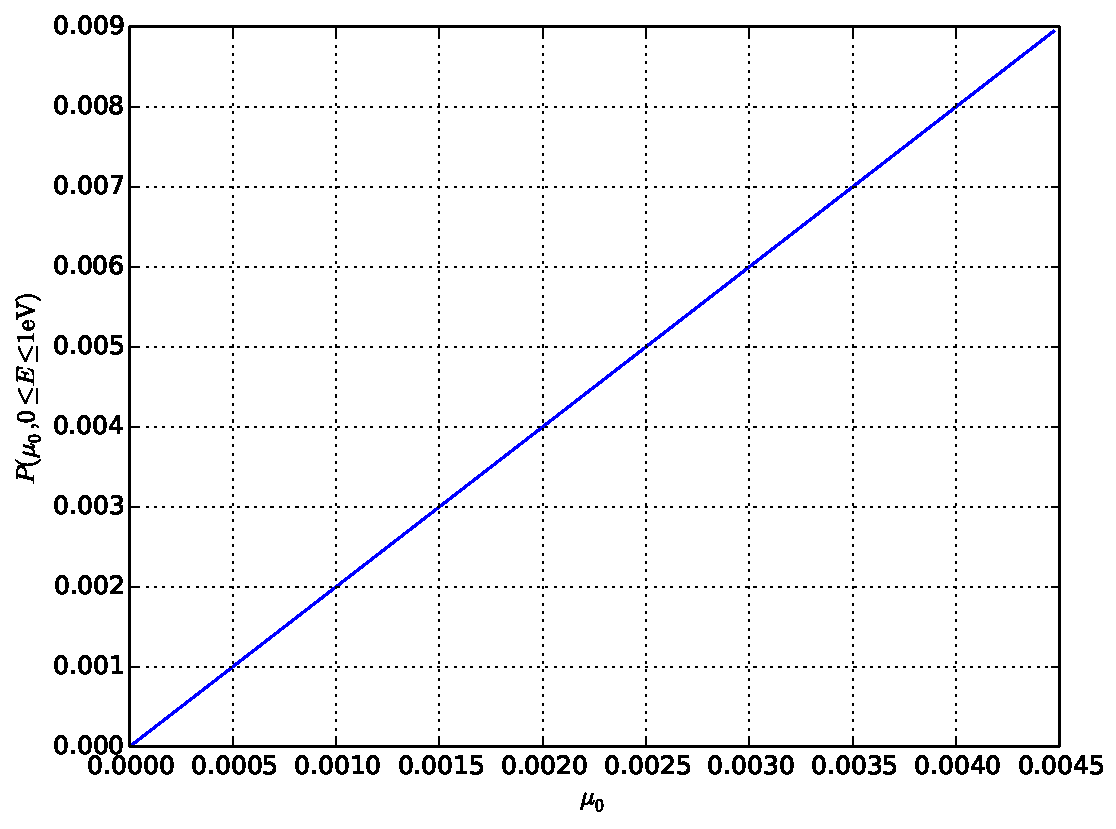
\includegraphics[width=\textwidth]{scat_kernel_05.pdf}
    \caption{$P(\mu_0)$ vs $\mu_0$}
\end{subfigure}
    \begin{subfigure}{0.5\textwidth}
    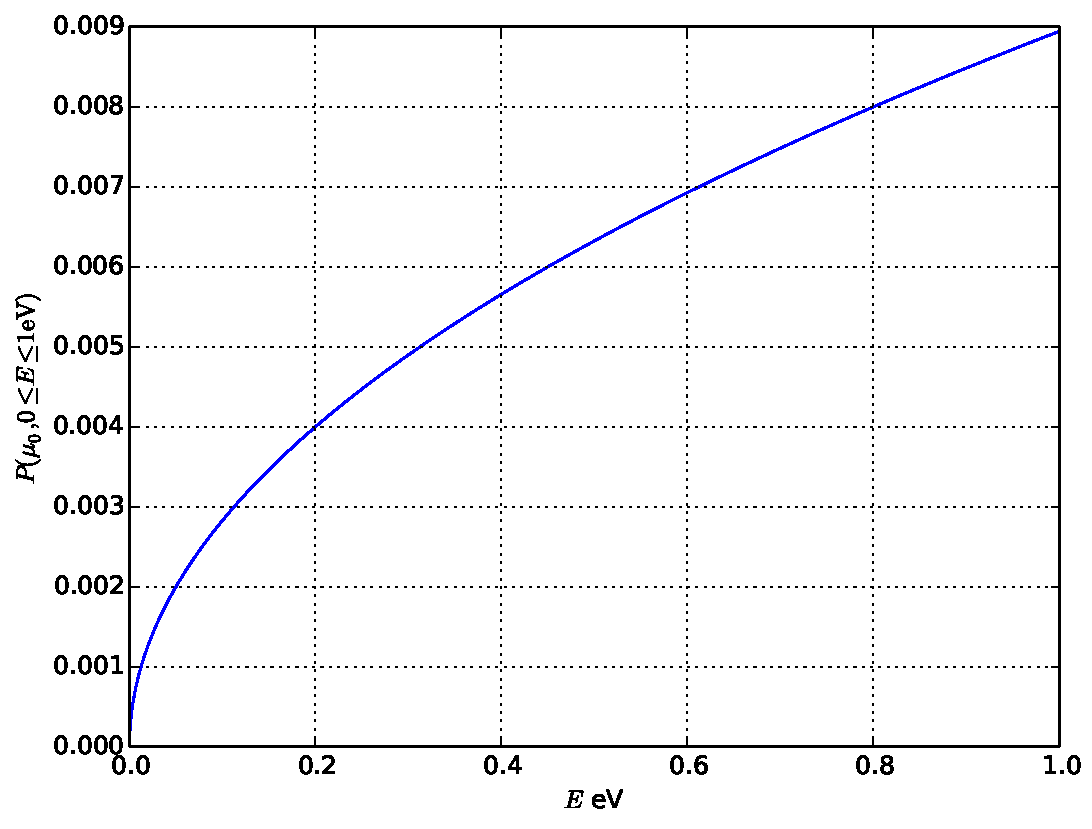
\includegraphics[width=\textwidth]{scat_kernel_E_05.pdf}
    \caption{$P(\mu_0)$ vs $E$}
\end{subfigure}
    \caption{Angular ditributions for $E'=0.05$ MeV}
\end{figure}
\begin{figure}
\begin{subfigure}{0.5\textwidth}
    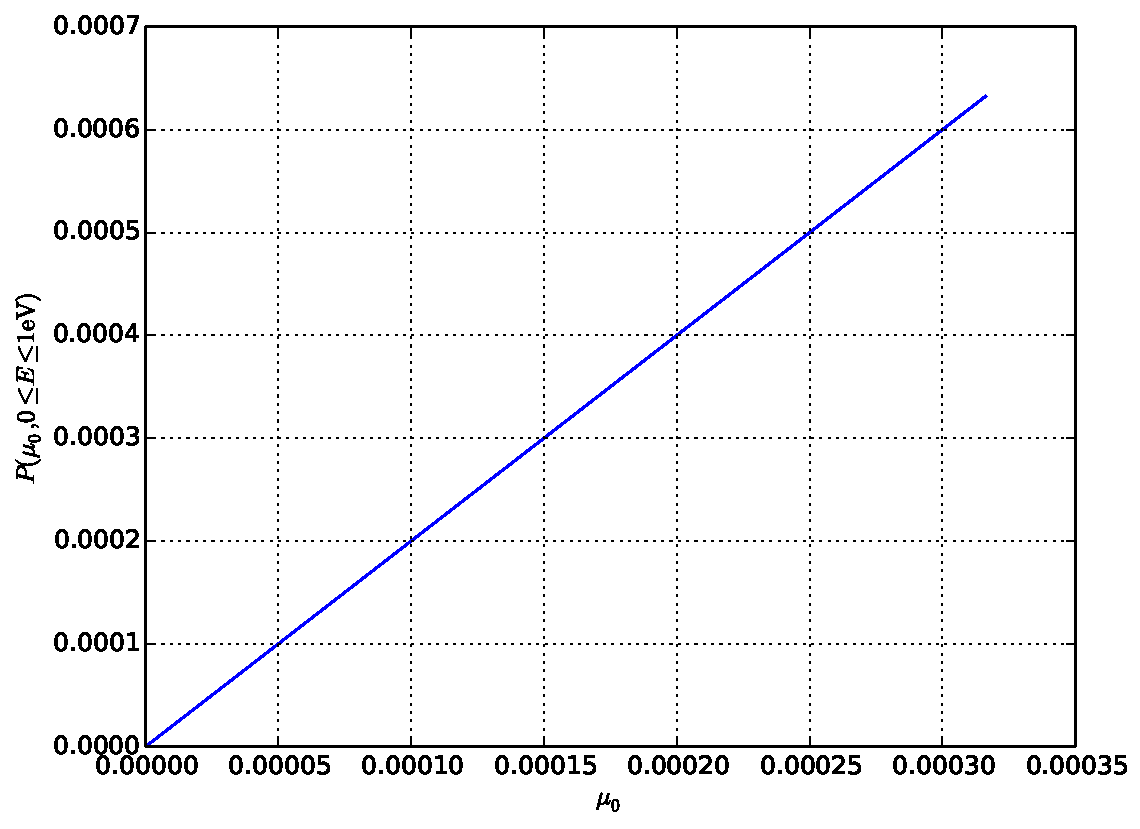
\includegraphics[width=\textwidth]{scat_kernel_10.pdf}
    \caption{$P(\mu_0)$ vs $\mu_0$}
\end{subfigure}
\begin{subfigure}{0.5\textwidth}
    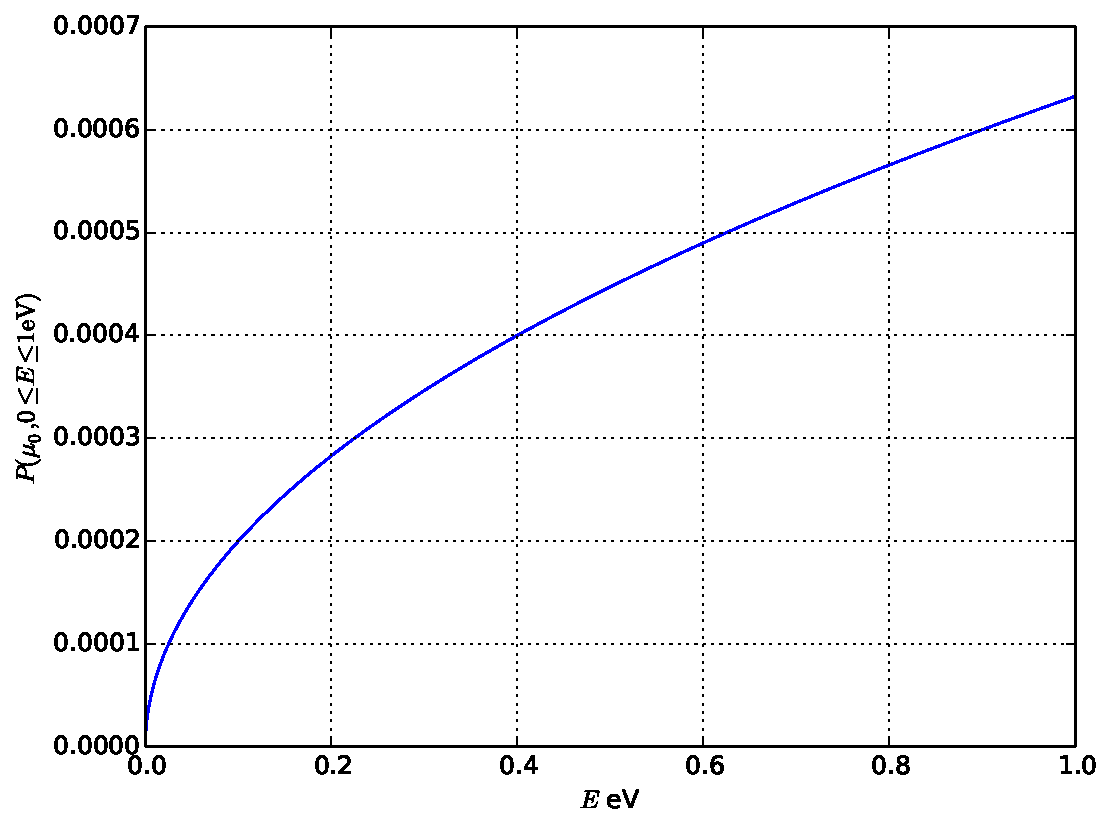
\includegraphics[width=\textwidth]{scat_kernel_E_10.pdf}
    \caption{$P(\mu_0)$ vs $E$}
\end{subfigure}
    \caption{Angular distributions for $E'=10$ MeV}
\end{figure}

 




 \end{solution}

 \begin{thebibliography}{9}

     \bibitem{dunnshultis}
         W.L. Dunn and J.K. Shultis, \emph{Exploring Monte Carlo Methods}, 2012.


\end{thebibliography}
\clearpage
\begin{problem}{3}
The problem details are given on the second page.
\end{problem}

\begin{solution}

\subsubsection*{Description of code}

The angular flux $\psi$ is computed by tracing characteristics as discussed in class.  To
compute points of intersection, the ray and surfaces of intersection are written in
parametric form. The position of a particle in the projected $x-y$ plane is denoted
$\mathbf{r} = x\ihat +
y\jhat$. Since we want to trace upstream, the parametric equation for the particle
position is given by 
\begin{equation}
    \mathbf{r} = (x_{i-1}-\Omega_xs)\ihat + (y_{i-1} - \Omega_ys)\jhat
\end{equation}
where $\mathbf{r}_{i-1}$ is the previous location, $s$ is a parameter that corresponds
to the signed distance the ray has traversed, and
\begin{align}
    \Omega_x =& \sin(\theta)\cos(\phi) \\
    \Omega_y =& \sin(\theta)\sin(\phi).
\end{align}
The parametric equation for each of the surfaces in the problem as a function of $x$ and
$y$ are given in Table~\ref{surfs}.  These equations are then evaluated with
$x=x_{i-1}-\Omega_xs$ and $y=y_{i-1}-\Omega_ys$ and solved for $s$ algebraically.
This produces a collection of values $\{s_m\}$, where $s_m$ represent the signed
distance to the $m$-th surface (excluding surfaces where a solution does not exist).
The smallest positive value of $s_m$ corresponds to the next point of intersection.  If we were already at a surface, then
that equation will give $s_m=0$.  Care is taken to exclude this solution, accounting
for potential roundoff.
\begin{table}[h]
    \centering
    \caption{Parametric equations for surfaces in problem.\label{surfs}}
    \begin{tabular}{|c|c|c|} \hline
    Surface & $f(x,y)=0$ \\ \hline
    Fuel    & $x^2 + y^2 - R_{\text{fuel}}^2=0$ \\
    Left Boundary & $x - x_{\min}=0$ \\
    Right Boundary & $x - x_{\max}=0$ \\ 
    Bottom Boundary & $y - y_{\min}=0$ \\
        Top Boundary & $y - y_{\max}=0$ \\ \hline
    \end{tabular}
\end{table}

The current position of the ray is updated, and the number of mean free paths
traveled $\tau_i=s_i\Sigma_{t}(x,y)$ along the $i$-th path is computed. The total number of MFP
traveled up to the latest point $s_i$ is accumulated as
$\tau_{\text{tot},i}=\sum_{k=1}^i \tau_k$. 

Because the transport equation is linear, we can consider the
contribution from each fuel element to the angular flux separately. If the $i$-th path
traced to point $\mathbf{r}_i$ was across a fuel element, then a contribution is made
to the flux.  If the path of length $s_i$ crossed the $j$-th fuel element, the contribution to the flux from that fuel element is
computed as
\begin{equation}\label{psij}
    \psi_j =
    \frac{Qe^{-\tau_{\text{tot},i-1}}}{4\pi\Sigma_{t,F}}\left(1-e^{-\Sigma_{t,F}s_i}\right)
\end{equation}
where $\tau_{\text{tot},i-1}$ does not include $s_i\Sigma_{t,F}$ because
that attenuation was accounted for in derivation of the term in parenthesis. The
ray tracing is then continued from this point until $\tau_{\text{tot,i}} >
\tau_{\max}$. 

Finally, after computing potential contributions to $\psi$, if the ray hits a boundary, the corresponding coordinate is
translated to the opposing boundary.  For example, if the right boundary is hit at
point $\mathbf{r}=x_{\max}\ihat+y_1\jhat$, the new position is $\mathbf{r} =
x_{\min}\ihat + y_1\jhat$. Tracing then continues as before, by computing new
distances to intersections, with $\hat{\Omega}$ unchanged.  Care is taken to handle roundoff issues and corners.  

The final solution for $\psi$, at
the location and direction of interest, will be 
\begin{equation}
    \psi(\mathbf{r},\hat{\Omega}) = \sum_{j}^{N_{\text{fuel}}} \psi_j
\end{equation}
where $N_{\text{fuel}}$ is the total number of fuel elements crossed during the ray
tracing.  The process outlined above is repeated for all equally spaced
$\phi\in[0,2\pi)$, for the polar angle and position of interest.

\clearpage
\subsubsection*{Results}

To verify the code works, the algorithm was modified to handle a source in the
moderator by evaluating Eq.~\eqref{psij} at every point, with $Q$ and $\Sigma_t$ the
same in all regions of the problem.  This was found to produce the expected answer of
$\psi = Q/4\pi\Sigma_t$ for all angles and positions tested.  It is noted that a
bug was found later after running this test, so this is not the most rigorous
verification test. 

Figures are given below for each of the desired points and directions
The results were found to have physically expected values. Comparing the plots at
$\theta=\pi/2$ and $\theta=\pi/8$, the latter results are more stretched with
slightly higher peaks and lower troughs.  This is expected as the fuel element will
appear more elliptic to the point of interest.  For the case of (0.63,0.63), symmetry
in the 4 quadrants appeared as expected. The largest values of
the flux, with the same magnitude, were found at $\phi=\pi/4,3\pi/4,5\pi/4$, and
$7\pi/4$; these are the points where the rays cross the entirety of the fuel
circumference.  The values of 0 at factors of $\pi/2$ were also seen as expected. This is
the only angle where no fuel tracks to the spatial location. At slightly different angles, a fuel pin is
hit at some point due to the limited attenuation by the moderator. In the other
plots, the expected relative magnitudes of the flux in the different quadrants were
seen as expected.  For instance, at (0.41,0.41), in $[0,\pi/2]$ there is a
similar shape as from $[\pi,3\pi/2]$, but in larger magnitude. The extra edges near
$0$ and $\pi/2$ occur because the ray sees most of the next fuel element past the one
it is nearest to, however this does not occur in $[\pi,3\pi/2]$.
As an additional verification, the code was compared against other students' codes who developed
algorithms independently and were found to agree.  Although this is not proof the
solution method is correct, it indicates that the code is implemented as intended.

It was found that at 8000 values of $\phi$ there was no visible difference in the
results.  A plot of one case for 8000 and 800 directions can be seen below in
Fig.~\ref{8000}. There are still a few points that are not picked up at 800
directions.  

\begin{figure}
    \begin{subfigure}{0.5\textwidth}
\centering
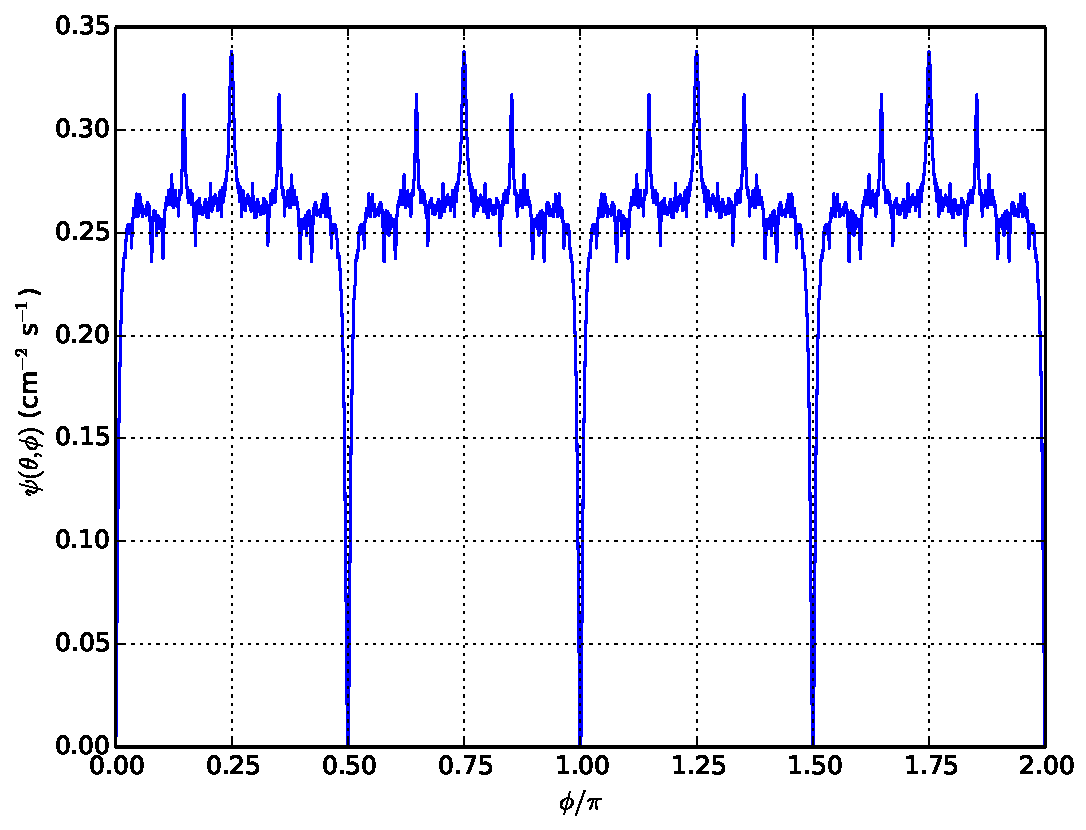
\includegraphics[width=1.0\textwidth]{r6363pi2.pdf}
\caption{$\theta=\pi/2$}
    \end{subfigure}
    \begin{subfigure}{0.5\textwidth}
\centering
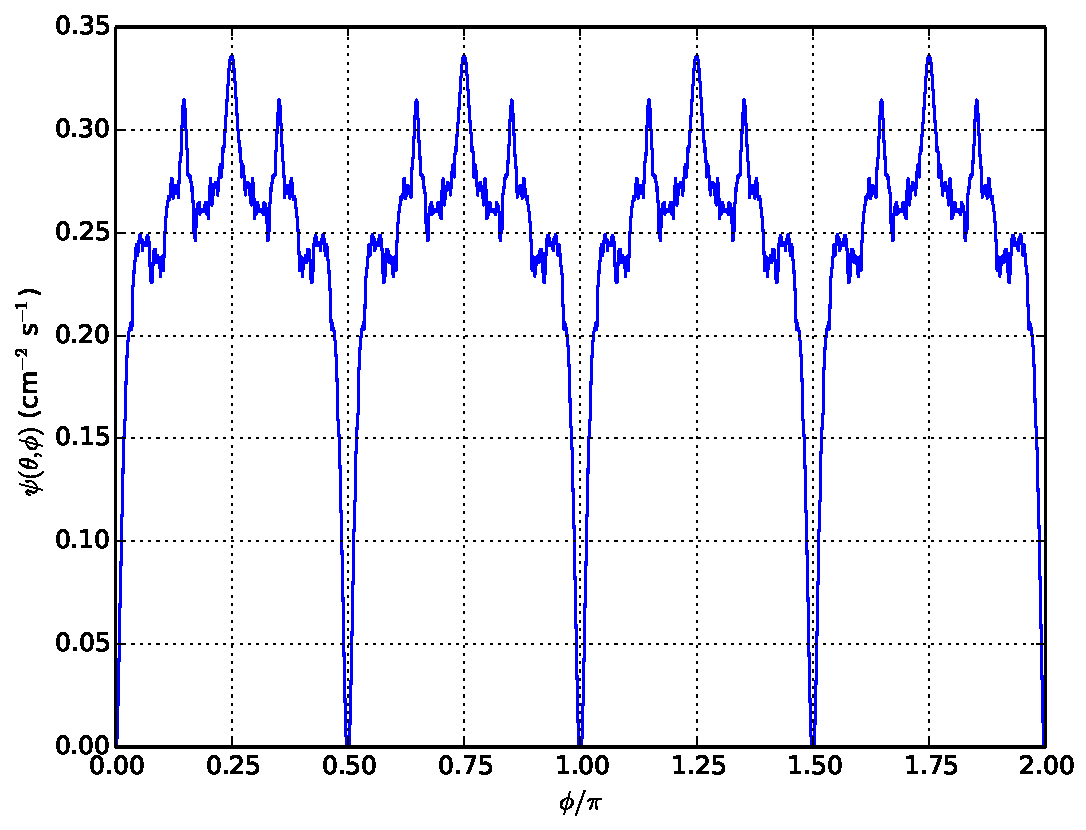
\includegraphics[width=1.0\textwidth]{r6363pi8.pdf}
\caption{$\theta=\pi/8$}
    \end{subfigure}
    \caption{Angular flux results at $x=0.63$ cm $y=0.63$ cm for 8000 azimuthal angles.}
\end{figure}
\begin{figure}
    \begin{subfigure}{0.5\textwidth}
\centering
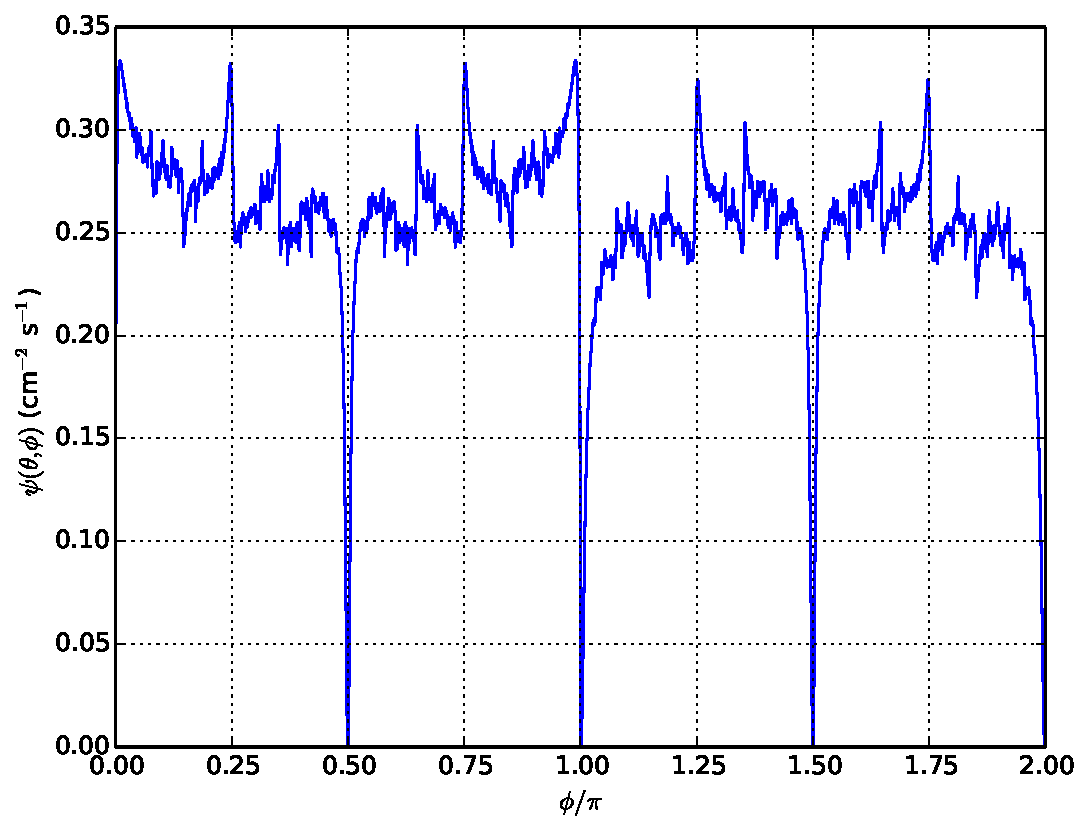
\includegraphics[width=1.0\textwidth]{r4163pi2.pdf}
\caption{$\theta=\pi/2$}
    \end{subfigure}
    \begin{subfigure}{0.5\textwidth}
\centering
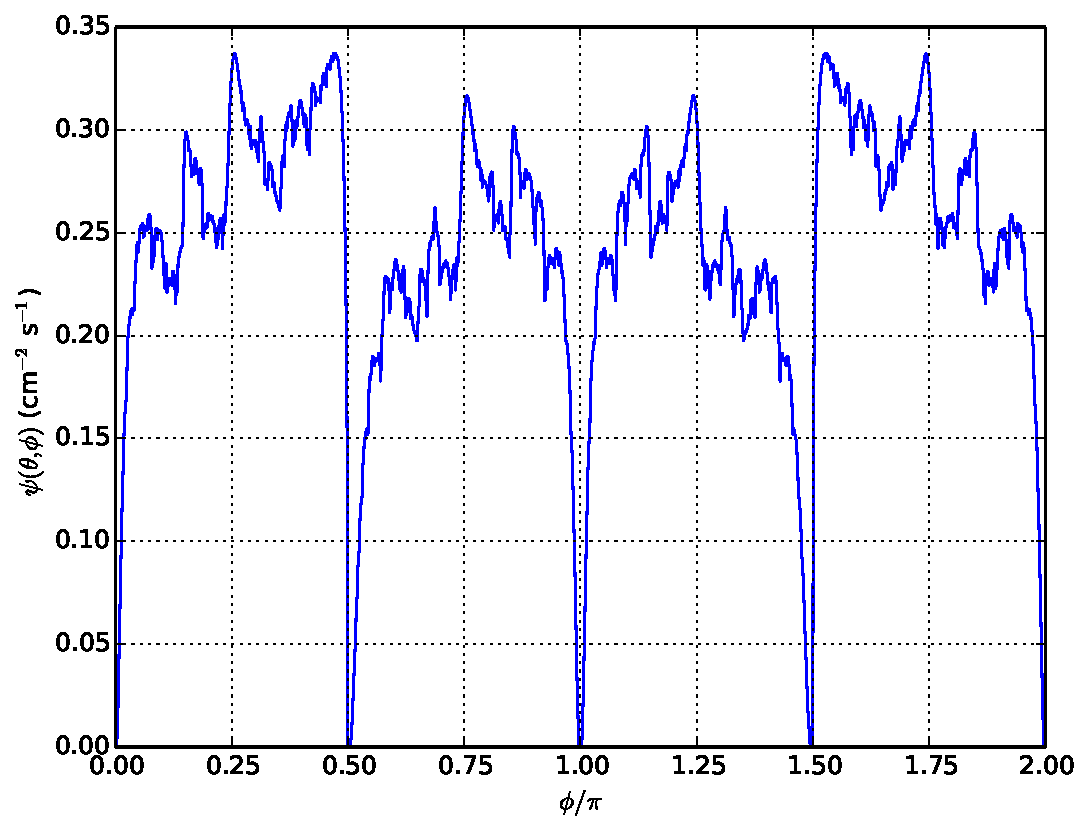
\includegraphics[width=1.0\textwidth]{r4163pi8.pdf}
\caption{$\theta=\pi/8$}
    \end{subfigure}
    \caption{Angular flux results at $x=0.63$ cm $y=0.41$ cm for 8000 azimuthal angles.}
\end{figure}
\begin{figure}
    \begin{subfigure}{0.5\textwidth}
\centering
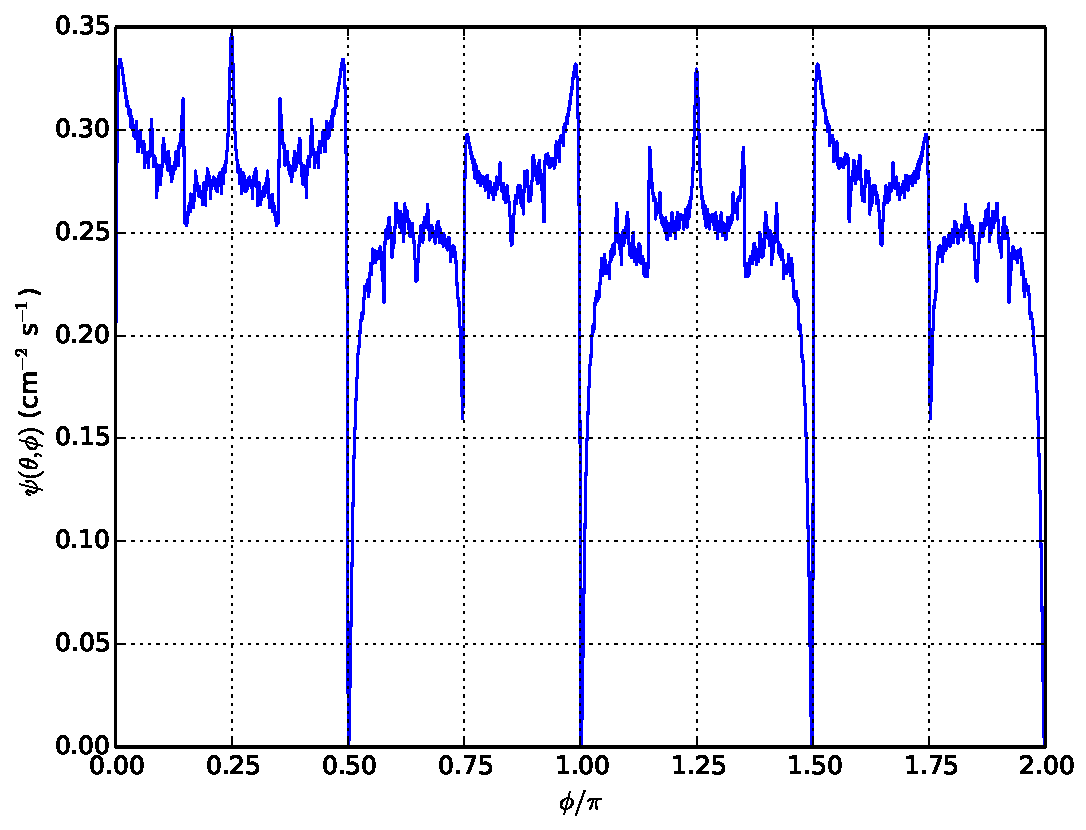
\includegraphics[width=1.0\textwidth]{r4141pi2.pdf}
\caption{$\theta=\pi/2$}
    \end{subfigure}
    \begin{subfigure}{0.5\textwidth}
\centering
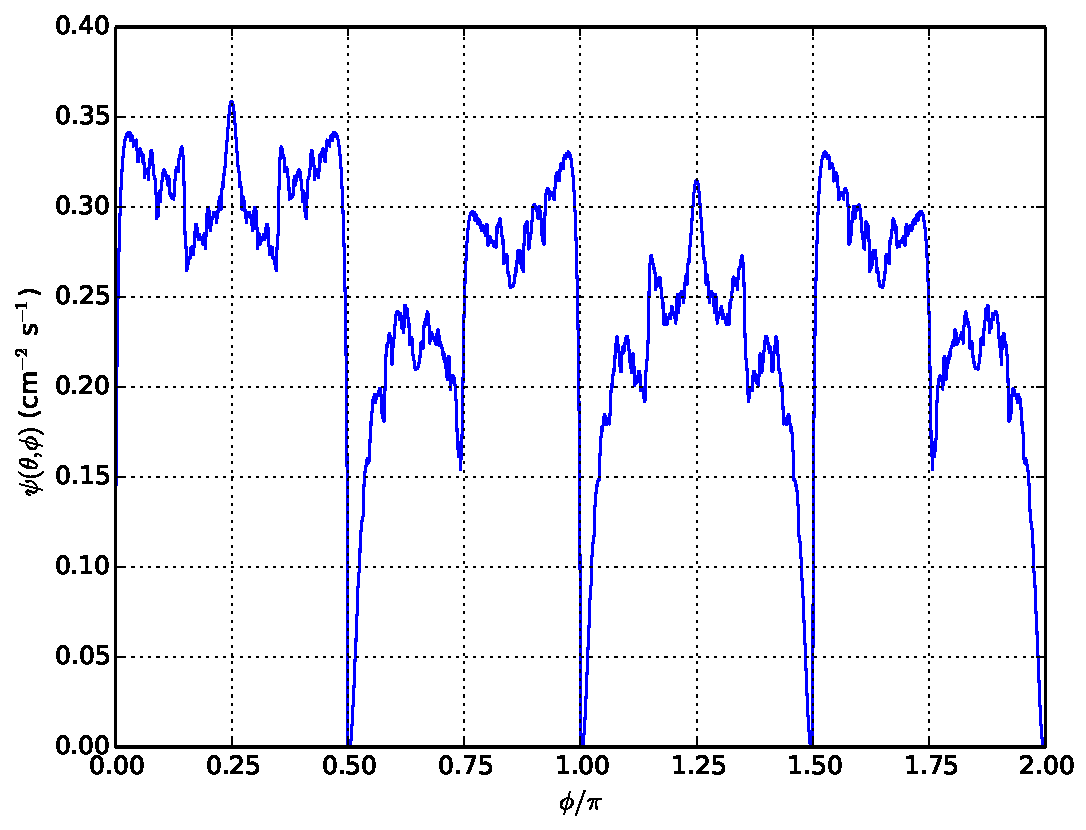
\includegraphics[width=1.0\textwidth]{r4141pi8.pdf}
\caption{$\theta=\pi/8$}
    \end{subfigure}
    \caption{Angular flux results at $x=0.41$ cm $y=0.41$ cm for 8000 azimuthal angles.}
\end{figure}


\begin{figure}
    \begin{subfigure}{0.5\textwidth}
\centering
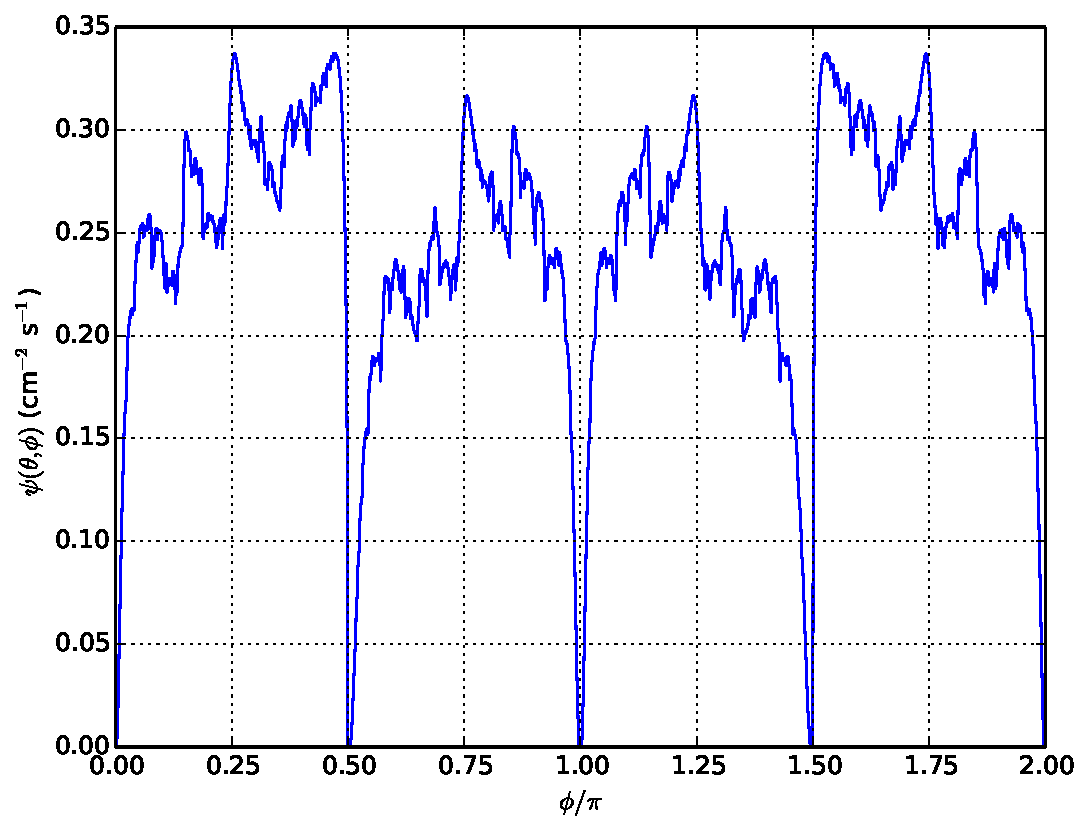
\includegraphics[width=1.0\textwidth]{r4163pi8.pdf}
\caption{8000 azimuthal angles}
    \end{subfigure}
    \begin{subfigure}{0.5\textwidth}
\centering
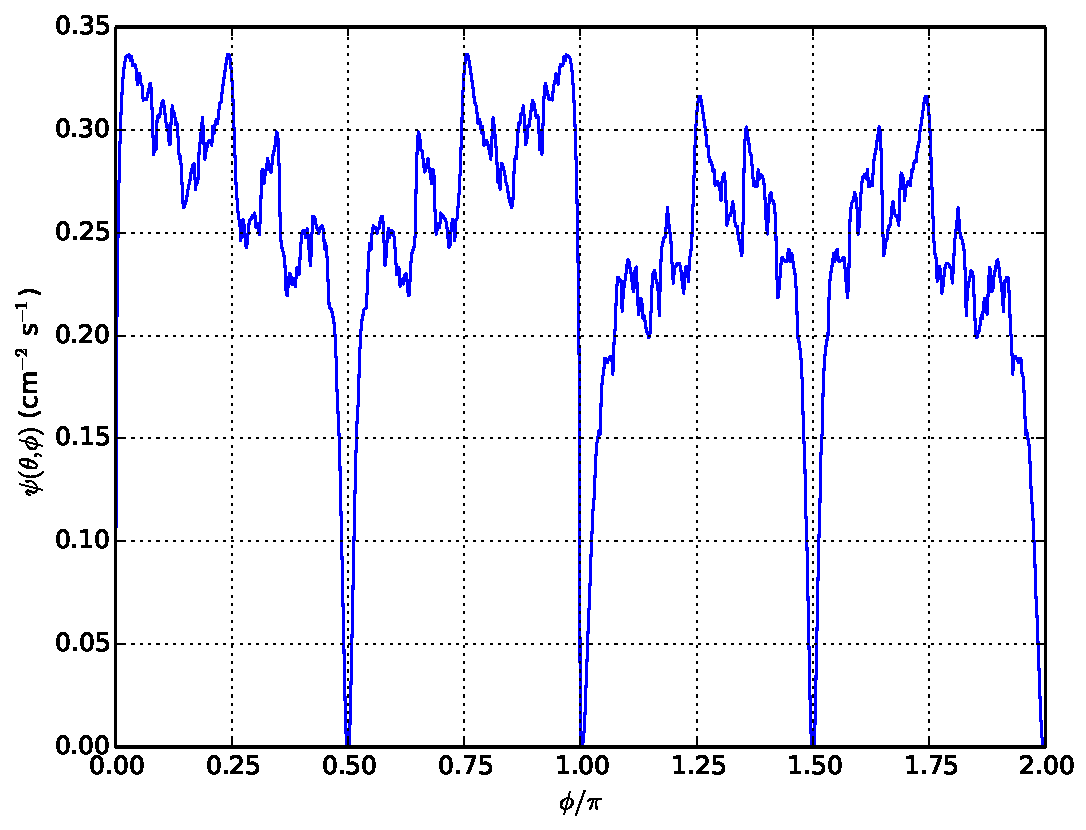
\includegraphics[width=1.0\textwidth]{800.pdf}
\caption{800 azimuthal angles.}
    \end{subfigure}
    \caption{\label{8000}Angular flux results at $\theta=\pi/8$, $x=0.63$ cm, and $y=0.41$ cm.}
\end{figure}

\clearpage
\lstinputlisting[basicstyle=\scriptsize]{moc_code/moc_pureabsorber.py}

\end{solution}


\end{document}



